\documentclass[12pt,twoside]{article}
\usepackage{paperstyle}  % Loads my formatting 
\usepackage{booktabs}
%\usepackage{tweaklist}  % I use this package as well; you may need to download

%% Shortcut commands
%\newcommand{\proptitle}[1]{\color{TaylorBlue} \textnormal{(#1):}}
%\newtheorem{proposition}{\color{TaylorGreen} Proposition}
%\newcommand{\assume}[2]{{\bf{Assumption #1}} (#2)} 
%\newcommand{\clr}[1]{{\color{TaylorBlue} #1}}
%\newcommand{\clrg}[1]{{\color{TaylorGreen} #1}}
%\newcommand{\Proof}[2]{\newline {\hspace{-\parindent} {\color{TaylorGreen}\bf Proof of Proposition}~\ref{#1}.}{\color{TaylorBlue} #2} \vspace{.1in}}
% If you've loaded *tweaklist.sty* above, uncomment these lines:
% Adjust spacing in itemize/enumerate; see tweaklist.sty
%\renewcommand{\enumhook}{\setlength{\topsep}{2pt}%
%  \setlength{\itemsep}{0pt}}
%\renewcommand{\itemhook}{\setlength{\topsep}{2pt}%
%  \setlength{\itemsep}{0pt}}

\begin{document}
\bibliographystyle{aernobold}

%%%%%%%%%%%%%%%%%%%%%%%%%%%%%%%%%%%%%%%%%%%%%%%%%%%%%%%%%%%%%%%%%
% TITLE PAGE
%%%%%%%%%%%%%%%%%%%%%%%%%%%%%%%%%%%%%%%%%%%%%%%%%%%%%%%%%%%%%%%%%

%\begin{singlespacing}
\begin{spacing}{0.6}
\begin{titlepage}

\title{Long Run Market Access and the Rise of the Sunbelt\thanks{People to thank...}}
\runningheads{}{}

\author{\normalsize\href{http://jaworskit.github.io}{Taylor 
	Jaworski}\\{\footnotesize Univ of Colorado, Boulder \& NBER} \and \normalsize\href{https://sites.google.com/site/kitchct/}{Carl 
	Kitchens}\\{\footnotesize Florida State Univ \& NBER}
   }

\date{\small \today}
\maketitle
\thispagestyle{empty}
\setcounter{page}{0}

%\clearpage
%\vspace{-0.3in}

\begin{abstract}
   Abstract goes here...
\end{abstract}

\end{titlepage}
\end{spacing}
%\end{singlespacing}


%%%%%%%%%%%%%%%%%%%%%%%%%%%%%%%%%%%%%%%%%%%%%%%%%%%%%%%%%%%
\section{Introduction}
%%%%%%%%%%%%%%%%%%%%%%%%%%%%%%%%%%%%%%%%%%%%%%%%%%%%%%%%%%%

\begin{itemize}
	\item Introduction
	
	\item Historical Background
	
	\item Data and Summary Statistics
	
	\item Empirical Analysis and Results
	\begin{itemize}
		\item Urban wage premium, number of workers, and market access
		\begin{itemize}
			\item relative to housing values			
		\end{itemize}
		
		\item Urban skill premium, number of workers, and market access
		
	\end{itemize}
\end{itemize}
	


% --------------------------------------------------
\section{Data}
% --------------------------------------------------

For our individual-level data, we use the IPUMS Full Count Census for 1940, the 1\% Sample for 1950, 1960-2000 5\% Census Samples Census, and 2005, 2010, and 2015 American Consumer Survey data. Our sample consists of adult men living in the continental US between the ages of 25 and 65 who are employed for at least 26 weeks in the sample year. We apply IPUMS person weights in all our regressions. 

We compute average weekly wages by finding total income divided by the number of weeks worked in the given survey year. For individuals earning the top income code, we set their total income to $1.5 \times$ the top income lower cutoff.\footnote{These cutoffs are reported in IPUMS INCWAGE documentation. In 2015 \$, the cutoffs are \$84,500 for 1940, \$99,2000 for 1950, \$199,500 for 1960, \$309,000 for 1970, and \$225,000 for 1980. Afterwards, IPUMS reports income as the median wage above that year's cutoff.} If the urban wage premium is primarily driven by people in the top income group, our estimates of the urban wage premium will be biased downwards. All incomes are then multiplied by the Consumer Price Index to be in 2015 dollars. In order to have a consistent measure of occupation, we use the `occ1950' variable provided by IPUMS which harmonizes occupation codes across all our survey years.


% --------------------------------------------------
\subsection{Market Access}
% --------------------------------------------------

Our measure of market access comes from a model of inter-regional trade introduced in \citet{Eaton_Kortum_2002}, \citet{Redding_Venables_2004}, and \citet{Donaldson_Hornbeck_2016}. A county $c$'s market access, $MA_c$, is given by this system of non-linear equations \[
    MA_{c} = \rho \sum_d \tau_{cd}^{-\theta} MA_d^{-1} Y_d,
\]
where $\theta$ is the trade elasticity with respect to trade costs, $\rho$ is a constant from the theoretical model, and $Y_d$ is the income of county $d$ measured by GDP. 

Our measure of the iceberg trade costs to ship from county $c$ to county $d$ in year $t$, $\tau_{cd}$, measures the fuel costs to travel to a county $d$ as well as the wage paid to the truck driver for the drive time. The formula for $\tau_{cdt}$ is given by \begin{align*}
    \tau_{cdt} &= \text{distance in miles}_{cdt} \times \text{cost per mile}_t \\
    &\quad + \text{travel time in hours}_{cdt} \times \text{hourly wage of truck drivers}_t
\end{align*} 
    
To create this measure of inter-regional trade costs, $\tau_{cd}$, we use digitized highway maps from 1940, 1950, 1960, 1970, 1980, 1990, 2000, and 2010 which include info on distance and the speed-limit of highway segments. For 2005 and 2015, we use our 2000 and 2010 highway maps respectively. Our measure, formed by finding the lowest-cost path, incorporates both the distance traveled and the speed of the highway.\footnote{More details on how the trade costs are calculated can be found in Section III of \citet{Jaworski_Kitchens_2019}.} 

The market access variable summarizes a county c's access to the transportation network by taking an average of other counties' market size weighted by both the trade cost to ship to those markets and by all other counties access to that market ($MA_{d}^{-1}$). Therefore a county $c$'s market access is large when it has access to large markets that other counties have little access to.

To aggregate market access to Urban areas, we created a crosswalk of counties within MSAs. For each MSA, we average across the counties within the MSA.\footnote{Our results are robust to weighting by population. (NEED TO CHECK)} Our measure of non-urban market access for a given state is the average of counties in that state that do not fall within any MSA. Therefore, for each individual we have a measure of whether or not they live in an urban area and the market access of the urban/non-urban area they live in.

% --------------------------------------------------
\subsection{Summary Statistics}
% --------------------------------------------------

Summary statistics of our data is in Table \ref{table:summ}. The percentage of people living in urban areas has steadily increased over time from 66\% in 1940 to a high of 81\% in 2015. This trend matches those found in \citet{Boustan_Bunten_Hearey_2013}. The log of our market access measure also grows over time which can be explained by both improvements in transportation networks over time as well as growth in GDP. The last four columns of Table \ref{table:summ} show the wage among people living in MSAs versus those that work in nonurban areas. Both urban and nonurban mean weekly wages are growing over time in real terms from \$33.24 and \$25.23 in 1940 to \$1353.95 and \$1067.48 in 2015.


% Summary Statistics
\begin{table}[tb]
    \caption{Summary Statistics}
    \label{table:summ}

    \resizebox{\linewidth}{!}{
        \centering

        \begin{tabular}{@{\extracolsep{5pt}}lccrrrrrr}
        \toprule  
        & & & & & \multicolumn{2}{c}{Urban Weekly} & \multicolumn{2}{c}{Nonurban Weekly} \\
        & & & \multicolumn{2}{c}{$\log$(Market Access)} & \multicolumn{2}{c}{Wage (2015 \$)} & \multicolumn{2}{c}{Wage (2015 \$)} \\
        \cline{4-5} \cline{6-7} \cline{8-9}
        Year & N & \% Urban & Mean & SD & Mean & SD & Mean & SD \\ \hline 

        1940        &  16,939,585&        0.66&        3.39&        0.87&          33&          20&          25&          17\\
1950        &      68,457&        0.69&        3.38&        0.67&          72&          41&          59&          33\\
1960        &   1,364,970&        0.66&        3.33&        0.66&         124&          77&         100&          60\\
1970        &     280,338&        0.75&        3.42&        0.70&         205&         138&         166&         105\\
1980        &   1,910,440&        0.73&        3.22&        0.57&         409&         284&         341&         221\\
1990        &   2,262,149&        0.74&        3.12&        0.46&         701&         562&         558&         405\\
2000        &   2,583,088&        0.79&        3.08&        0.42&       1,008&       1,015&         767&         677\\
2005        &     530,737&        0.79&        3.08&        0.42&       1,143&       1,146&         863&         712\\
2010        &     530,783&        0.80&        3.01&        0.51&       1,228&       1,210&         961&         819\\
2015        &     561,934&        0.81&        3.00&        0.52&       1,353&       1,446&       1,068&       1,011\\


        \bottomrule

        \end{tabular}
    
    }
    
    \vspace{2mm}
    {\footnotesize
        \textit{Notes:} Weekly wage is reported in 2015 \$. Market Access is calculated from solving $MA_{c} = \rho \sum_d \tau_{cd}^{-\theta} MA_d^{-1} Y_d,$ where transportation costs, $\tau_{cd}$, are calculated as described in the text. 
    }
\end{table}

Figure \ref{fig:ma_dev_over_time} shows within-year deviations of the log of market access from the yearly mean. The figure shows that over time, non-urban areas have had a relative growth in market access, particularly in the western United States. On the other hand, large cities in the 1940 had very large market access relative to the national average and this relative advantage declines over time from about 4 log points to about 2 log points above the mean. The deviation in log market access reflects the variation used in our survey year regressions of the log of wage on the log of market access. 

Figure \ref{fig:ma_over_time} shows the log of market access over time. While Figure \ref{fig:ma_dev_over_time} showed that non-urban areas had relative growth in market access, this figure highlights that market access has been growing consistently through the 20th century in all areas. North Dakota in 2015, for example, has about the same level of market access of New York City in 1940. 


\begin{figure}[tb]
    \caption{Log of Market Access Deviations from Yearly Mean: 1940-2015}
    \label{fig:ma_dev_over_time}
    \centering
    
    \resizebox{\columnwidth}{!}{
        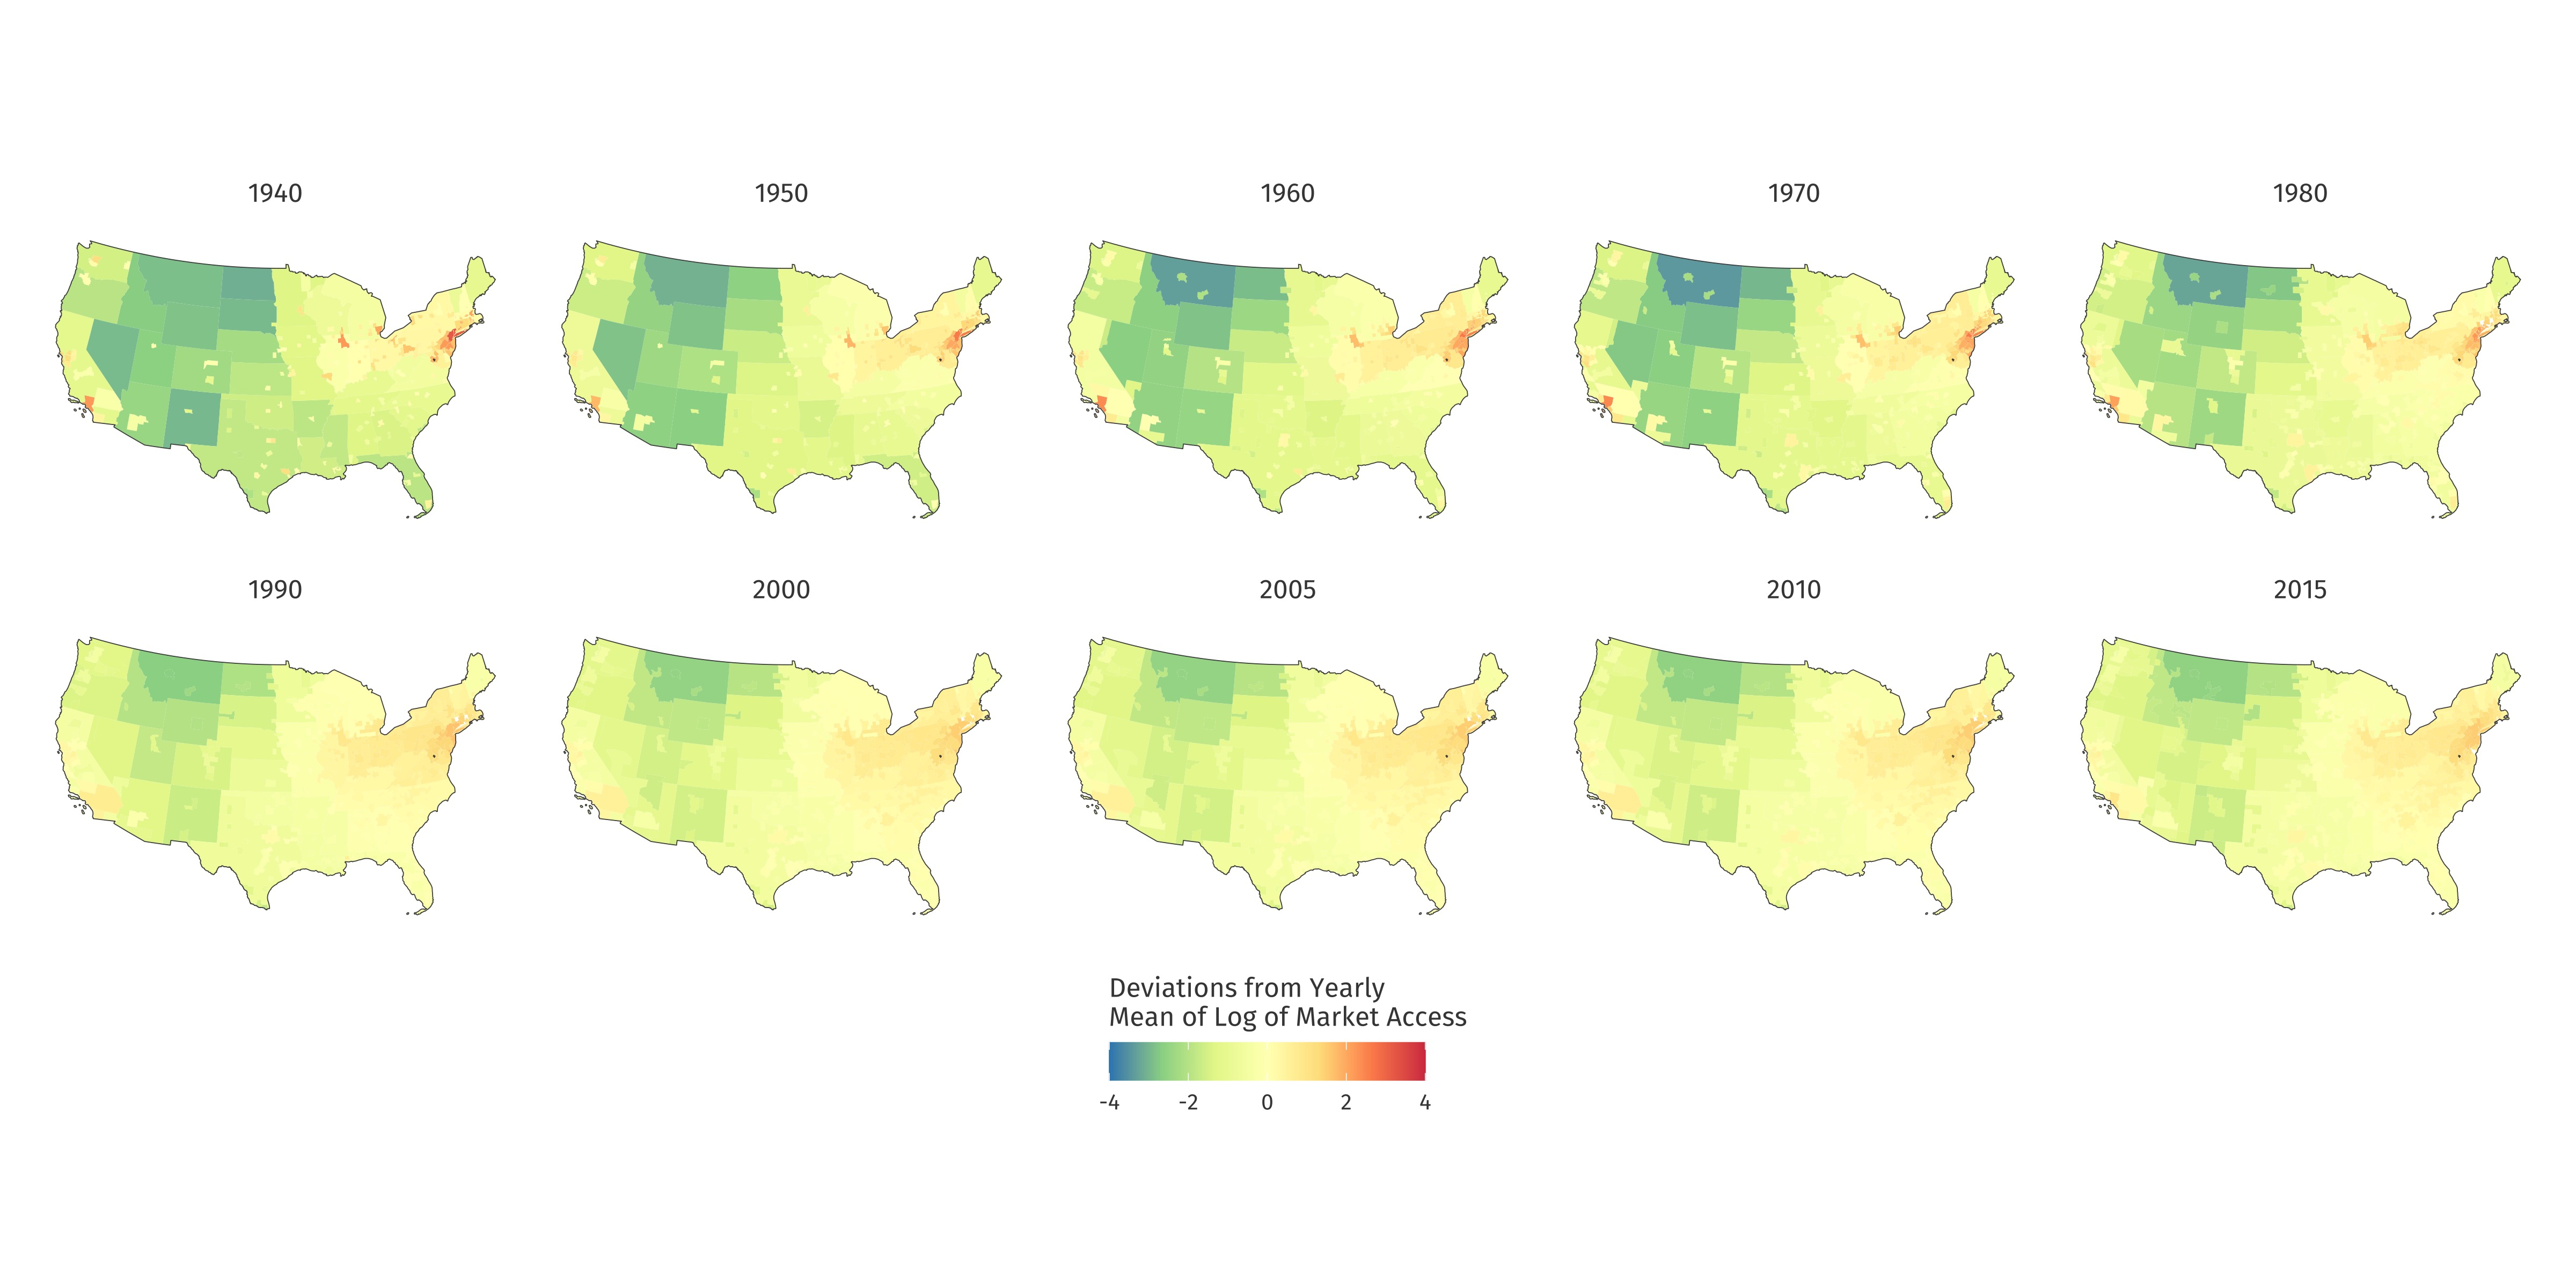
\includegraphics{figures/ma_deviations_over_time.jpg}
    } 
\end{figure}

\begin{figure}[tb]
    \caption{Log of Market Access over Time: 1940-2015}
    \label{fig:ma_over_time}
    \centering
    
    \resizebox{\columnwidth}{!}{
        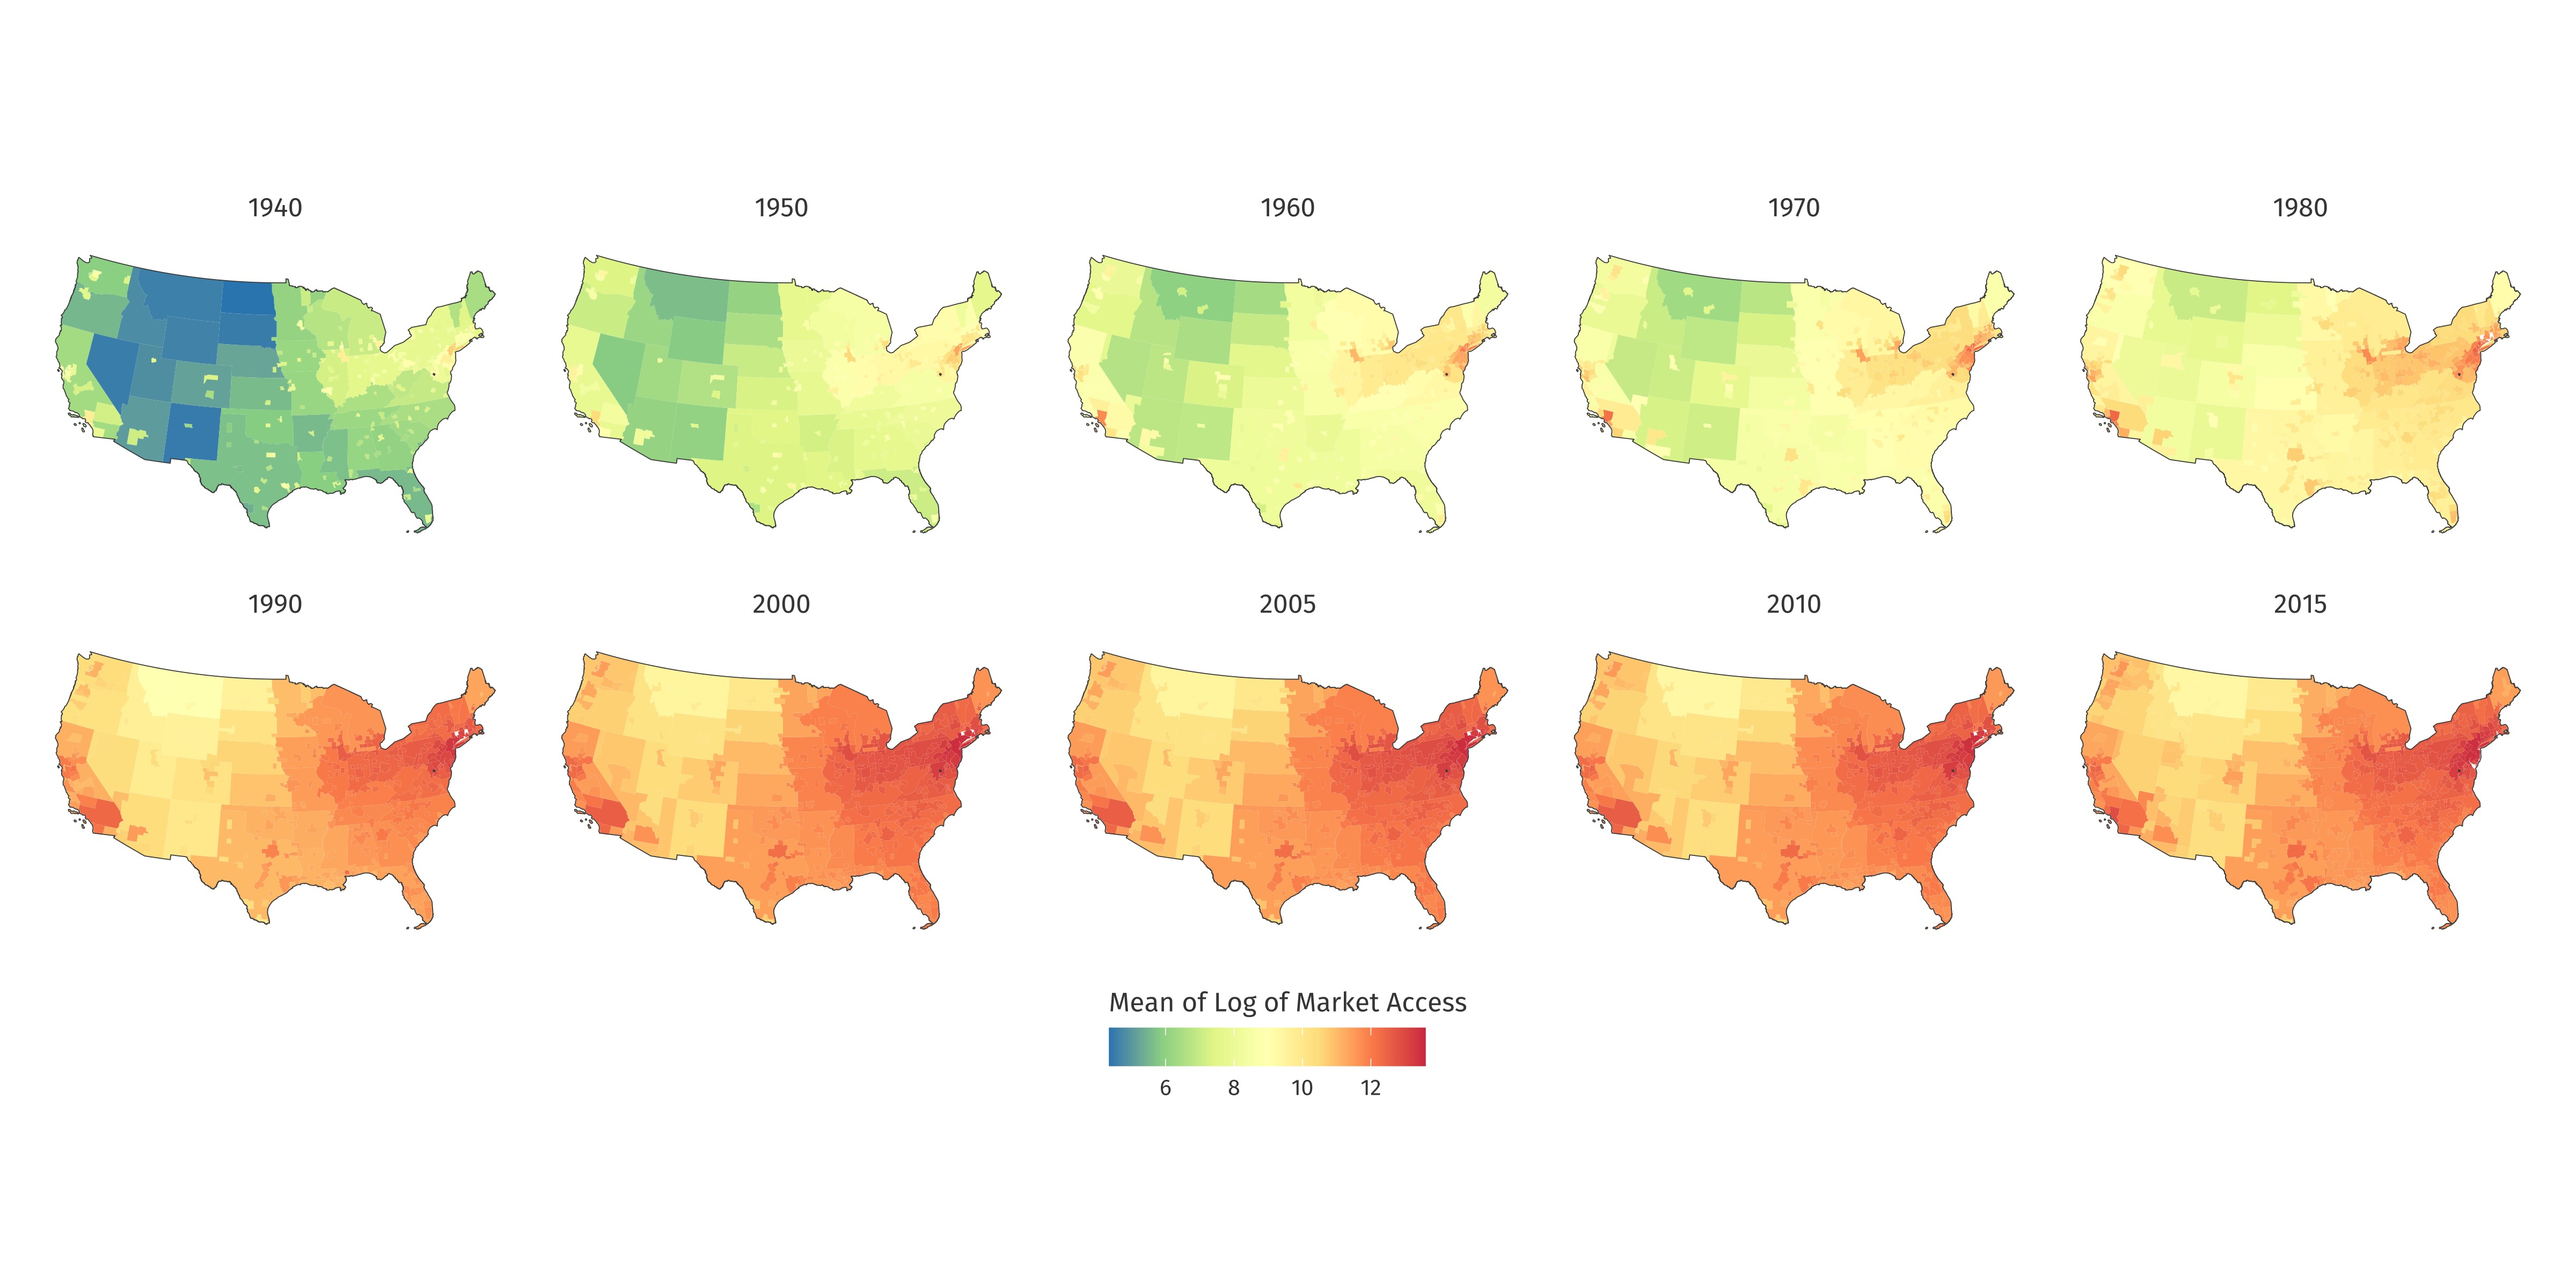
\includegraphics{figures/ma_over_time.jpg}
    } 
\end{figure}

@Question: For the map, there are some msas that are in the list we have but not showing up in the ipums data, should I use them still in the map?

@Question: Should there be a robustness check to prevent selection over time. If smaller and smaller MSAs are added, then we would expect a decline in wage premium even if the original cities' premium perhaps is growing. 
Also, it could be that our Market Access variable is picking up, in part, differences in the urban wage premium based on city size.



% --------------------------------------------------
\section{Results}
% --------------------------------------------------

For an initial understanding of the urban wage premium, for each survey year we take the average log-ratio between urban weekly wage and nonurban weekly wage. This replicates the method used in \citet{Boustan_Bunten_Hearey_2013}. In Figure \ref{fig:premium_over_time}, the `urban raw' line shows the results of this exercise. The U-shape in which the urban wage premium starts around 30\% in 1940, decreases between 1950 and 1980 to just over 20\% and then increases again to over 25\% after 2000 is consistent with results found in the literature.\footnote{Our resuts match the shape over time found in Figure 3 of \citet{Boustan_Bunten_Hearey_2013} while our estimate in 2000 is a few percentage points lower than the estimate of 32\% from \citet{Glaeser_Mare_2001}. The increase between 1980 and 2000 matches \citet{Baum-Snow_Pavan_2012}.}

Moving into a regression framework, we run versions of the following specification seperately for each survey year: \[
    \log(\text{Weekly Wage}_i) = \beta_0 + \beta_1 \text{Urban}_i + \beta_2 \log(\text{Market Access}_{MSA(i)}) + \delta X_{i} + \epsilon_i,
\]
where $X_i$ is a set of controls consisting of age in 5-year bins, education levels, and an indicator for being White. Our estimate of $\beta_1$ is the percent increase in wages that workers in urban areas have on average which we call the ``Urban Wage Premium''. The first version, `urban only', consists does not include the log of Market Access or controls $X_i$. This is the regression based version of the `urban raw' approach. However, there can be demographic differences between urban and rural areas that contribute to wage differentials and so we add controls for education, race, and age in the `urban w/ controls' specification. 

The wages of individuals in Urban areas also benefit from the improved transportation network, so in the final specification, `urban w/ market access', we add in the log of Market Access. After controlling for market access, the coefficient on Urban, $\beta_1$ should pick up on the non-transportation causes of the urban wage premium.\footnote{This includes the improved human capital development from \citet{Glaeser_Mare_2001} and improved firm-worker matching found in \citet{Baum-Snow_Pavan_2012}.} 

Our estimates for the urban wage premium will be biased if there is sorting into cities by characteristics that are correlated with wages but seperate from age, race, and education. An example could be that workers sort into cities based on the industry they work in and differences in industrial wages can explain some of the remaining wage premium. \citet{Combes_Duranton_Gobillon_2008} show using panel data that individual fixed effects remove a portion of the variation in urban wage premium. Our time-series data is cross-sectional, so we can not use individual level fixed effects in our estimation. For our estimates to be causal, the exclusion restriction requires there to be no sorting beyond age, race, and education levels. 

\begin{figure}[tb]
    \caption{Urban Wage Premium 1940-2015}
    \label{fig:premium_over_time}
    \centering
    
    \resizebox{\columnwidth}{!}{
        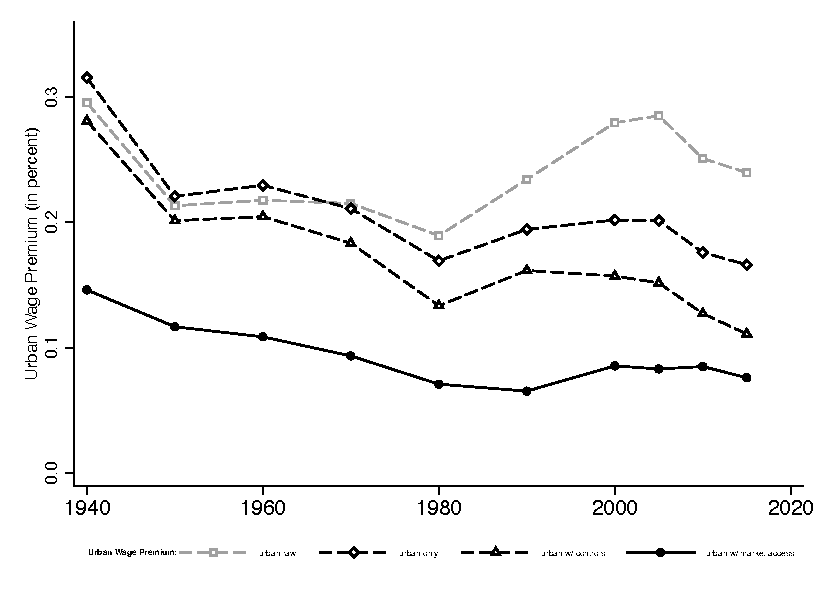
\includegraphics{figures/urbanpremium_IPUMS.pdf}
    } 
\end{figure}

The results from the regressions that do not include a measure of market access is found in Figure \ref{fig:premium_over_time} as the `urban only' and `urban w/ controls' lines. All regression tables can be found in Table \ref{table:ma_reg_all}. These lines show that the urban wage premium still decreases from a premium of around 30\% in 1940 through 1980. However, instead of the increase in the modern economy, our regression-based results show that the urban wage premium roughly levels off after 1980 at 20\% without controls and at around 16\% when controlling for age, education, and race. This result suggests that increased sorting of high-income earning people into cities can explain the recent increase in urban wage premium found in the raw-measures.

The final specification includes market access in the regression of the log of weekly wage on an urban indicator variable. This specification controls for the benefits cities receive from being located in an advantageous transportation network. If part of the wage premium is explained by better location in the transportation network, we expect the premium to decrease when including market access which summarizes the network. The estimates on the urban indicator are found in Figure \ref{fig:premium_over_time} as the `urban w/ market access' line and in Table \ref{table:ma_reg}. 

When controlling for the transportation advantage of cities, we see the urban indicator in 1940 has decreased to about 15\% from the 30\% observed in specifications that don't include market access. There still exists, albeit a much smaller, decline in urban wage premium through the 80s which flattens out to an urban wage premium of around 10\% that lasts until at least 2015. 

This result suggests that between 25.9\% to 47.7\% of the urban wage premium is explained by a relatively strong position in the transportation network.\footnote{The \% change in the urban wage indicator between `urban w/ control' and `urban w/ market access' is 47.7\% for 1940, 30.7\% for 1950, 35.9\% for 1960, 46.2\% for 1970, 35.4\% for 1980, 37.4\% for 1990, 26.1\% for 2000, 25.8\% for 2005, 33.1\% for 2010, and 27.4\% for 2015.} In particular, it appears that early in our sample, the differences in access to transportation network was large between urban and rural areas. This matches that historical highway networks focused on connecting large cities and starting around 1955 began connecting many more places which increased market access for rural areas. 

% MA Regression
\begin{table}[tb]
    \caption{Urban Wage Premium Estimates by Survey Year}
    \label{table:ma_reg}

    \resizebox{\linewidth}{!}{
        \centering

        \begin{tabular}{@{\extracolsep{5pt}}lrrrrrrrrrr}
        \toprule

        & \textbf{1940} & \textbf{1950} & \textbf{1960} & \textbf{1970} & \textbf{1980} & \textbf{1990} & \textbf{2000} & \textbf{2005} & \textbf{2010} & \textbf{2015} \\
        \cline{2-11}

        Urban     &   0.147&   0.137&   0.130&   0.098&   0.086&   0.100&   0.116&   0.112&   0.085&   0.076\\
          & (0.010)& (0.012)& (0.011)& (0.011)& (0.011)& (0.011)& (0.011)& (0.011)& (0.014)& (0.017)\\
$\log(MA)$&   0.053&   0.035&   0.051&   0.056&   0.038&   0.093&   0.070&   0.068&   0.067&   0.054\\
          & (0.003)& (0.007)& (0.010)& (0.009)& (0.010)& (0.011)& (0.010)& (0.013)& (0.015)& (0.016)\\
\hline N  &16,939,585&  68,457&1,364,970& 280,338&1,910,440&2,262,149&2,583,088& 530,737& 530,783& 561,934\\


        \bottomrule
        \end{tabular}
    
    }
    
    \vspace{2mm}
    {\footnotesize
        \textit{Notes:} Each cell is the coefficient estimate corresponding to the regression that includes log of market access from the sample year indicated by the column label.
    }
\end{table}





% --------------------------------------------------
\newpage 
{\small \bibliography{Growth.bib} }
% --------------------------------------------------


% --------------------------------------------------
\newpage \appendix
\renewcommand{\thetable}{\Alph{section}.\arabic{table}}
% --------------------------------------------------


% --------------------------------------------------
\section{Full Urban Wage Premium Regressions}
\setcounter{table}{0}
\setcounter{figure}{0}
% --------------------------------------------------

\begin{table}[tb]
    \caption{All Urban Wage Premium Estimates by Survey Year}
    \label{table:ma_reg_all}

    \resizebox{\linewidth}{!}{
        \centering

        \begin{tabular}{@{\extracolsep{5pt}}lrrrrrrrrrr}
        \toprule

        & \textbf{1940} & \textbf{1950} & \textbf{1960} & \textbf{1970} & \textbf{1980} & \textbf{1990} & \textbf{2000} & \textbf{2005} & \textbf{2010} & \textbf{2015} \\
        \cline{2-11}

        \multicolumn{11}{l}{\textbf{Panel A: Urban only}} \\
        Urban                    &      0.3153&      0.2208&      0.2295&      0.2109&      0.1692&      0.1943&      0.2018&      0.2014&      0.1759&      0.1661\\
                         &    (0.0177)&    (0.0131)&    (0.0135)&    (0.0119)&    (0.0110)&    (0.0157)&    (0.0144)&    (0.0160)&    (0.0165)&    (0.0175)\\
\hline N                 &  16,939,585&      68,457&   1,364,970&     280,338&   1,910,440&   2,262,149&   2,583,088&     530,737&     530,783&     561,934\\

        

        \midrule
        \multicolumn{11}{l}{\textbf{Panel B: Urban with Controls}} \\
        Urban                    &      0.2808&      0.2012&      0.2045&      0.1833&      0.1334&      0.1615&      0.1571&      0.1517&      0.1272&      0.1108\\
                         &    (0.0170)&    (0.0125)&    (0.0123)&    (0.0119)&    (0.0116)&    (0.0162)&    (0.0125)&    (0.0131)&    (0.0135)&    (0.0137)\\
\hline N                 &  16,939,545&      68,457&   1,364,970&     280,338&   1,910,440&   2,262,149&   2,583,088&     530,737&     530,783&     561,934\\



        \midrule
        \multicolumn{11}{l}{\textbf{Panel C: Urban, Controls, and Market Access}} \\
        Urban     &   0.147&   0.137&   0.130&   0.098&   0.086&   0.100&   0.116&   0.112&   0.085&   0.076\\
          & (0.010)& (0.012)& (0.011)& (0.011)& (0.011)& (0.011)& (0.011)& (0.011)& (0.014)& (0.017)\\
$\log(MA)$&   0.053&   0.035&   0.051&   0.056&   0.038&   0.093&   0.070&   0.068&   0.067&   0.054\\
          & (0.003)& (0.007)& (0.010)& (0.009)& (0.010)& (0.011)& (0.010)& (0.013)& (0.015)& (0.016)\\
\hline N  &16,939,585&  68,457&1,364,970& 280,338&1,910,440&2,262,149&2,583,088& 530,737& 530,783& 561,934\\


        \bottomrule
        \end{tabular}
    
    }
    
    \vspace{2mm}
    {\footnotesize
        \textit{Notes:} Each cell is the coefficient estimate corresponding to the regression that includes log of market access from the sample year indicated by the column label.
    }
\end{table}


% --------------------------------------------------
\section{MSA-level Market Access}
\setcounter{table}{0}
\setcounter{figure}{0}
% --------------------------------------------------

TODO: Include robustness for weighting MA by county population when aggregating






\end{document}